\documentclass[11pt]{article}
\usepackage{amsmath,amsfonts,amssymb,eucal,graphicx}
\usepackage{epsfig}
%\usepackage{pslatex}
\usepackage{wrapfig}
\usepackage{exscale}
\usepackage{setspace}
\usepackage{subfigure}
\usepackage{color}
\usepackage{url} 
\usepackage{float}
\restylefloat{table}
\usepackage{enumitem}
\usepackage{titlesec}
\titleformat*{\section}{\large\bfseries}
\titleformat*{\subsection}{\normalsize\bfseries}
\titleformat*{\subsubsection}{\large\bfseries}
\titleformat*{\paragraph}{\large\bfseries}
\titleformat*{\subparagraph}{\large\bfseries}
\usepackage[font=footnotesize]{caption}
\usepackage[letterpaper, margin=1in]{geometry}
%\usepackage{showframe}

\usepackage{cite}

\hyphenation{test-bed}

\textwidth  6.6in
\textheight 9.1in
\setlength{\oddsidemargin}{-0.04 in}
\setlength{\topmargin}{-0.7in}
\newcommand{\alex}[1]{\textcolor{cyan}{ #1}}
\newcommand{\noi}{\noindent}
\newcommand{\bi}{\begin{itemize}}
\newcommand{\ei}{\end{itemize}}
\newcommand{\bc}{\begin{center}}
\newcommand{\ec}{\end{center}}

\newcommand{\toc}{{\em IEEE Trans.~Communications, }}
\newcommand{\tit}{{\em IEEE Trans.~Information Theory, }}
\newcommand{\jsac}{{\em IEEE J. Selected Areas Commun., }}
\newcommand{\rtime}[1]{\par\noindent\rlap{#1} \hspace*{2.15cm}}
\newcommand{\iblank}{\par \noindent \hspace*{2.4cm} \hangindent 2.6cm}

\newcommand{\nm}[1]{\textcolor{red}{\textbf{[NM: #1]}}}
\newcommand{\ca}[1]{\textcolor{blue}{\textbf{[CA: #1]}}}
\newcommand{\as}[1]{\textcolor{cyan}{\textbf{[AS: #1]}}}

\def\etal{{\em et al.\/}}
\def\eg{{\em {\em e.g.},\ }}
\def\ie{{\em i.e.,\ }}
\def\etc{{\em etc.\ }}
\def\be{\begin{equation}}
\def\ee{\end{equation}}

\newcommand{\SNR}{{\sf SNR}}
\newcommand{\INR}{{\sf INR}}
\newcommand{\SINR}{{\sf SINR}}
\newcommand{\Nc}{{\cal N}}
\newcommand{\Ec}{{\cal E}}
 
 \newfont{\bb}{msbm10 scaled 1100}
\newcommand{\CC}{\mbox{\bb C}}
\newcommand{\PP}{\mbox{\bb P}}
\newcommand{\RR}{\mbox{\bb R}}
\newcommand{\QQ}{\mbox{\bb Q}}
\newcommand{\ZZ}{\mbox{\bb Z}}
\newcommand{\FF}{\mbox{\bb F}}
\newcommand{\GG}{\mbox{\bb G}}
\newcommand{\EE}{\mbox{\bb E}}
\newcommand{\NN}{\mbox{\bb N}}
\newcommand{\KK}{\mbox{\bb K}}

\renewcommand{\baselinestretch}{0.965}



\title{{\large\bf CIF21 DIBBS: PD: A Framework for Scalable Algorithm Sharing in Digital Agriculture}}

\author{
James V. Krogmeier,
Dennis R. Buckmaster,
Aaron C. Ault,
Charles Hillyer
}

\graphicspath{{./Figures/}}

\begin{document}

\noindent\textbf{\Large Project Description}\\

\section{Introduction} 
\label{sec:intro}

\subsection{Overview of Problem}
\label{ssec:OverviewOfProblem}

Today it is extremely difficult for researchers or companies in agriculture to use published or unpublished algorithms 
developed by others; many useful algorithms were written in antiquated coding languages or compiled for long-replaced 
operating systems. While principles of the algorithms were published in papers, often the code was not and attempts to 
recreate them are inefficient at best, and likely unsuccessful on average: "unsuccess" is rarely documented. For example, 
algorithms for soil erosion \cite{ARS:14}, whole farm modeling \cite{Rotz:16}, watershed delineation \cite{Djokic:00}, 
and pesticide risk assessment \cite{Antony:12} are "locked" in code that is largely inaccessible to and unusable by 
others in practice.  It is tedious and often difficult to tailor them to geo-referenced or high-resolution data which might be 
available.  While these and other tools like them have contributed to the research base in agriculture, few are used in 
production settings as decision aids; industry has had incomplete access which hinders the pool of new ideas and the ability 
of industry "on the ground" to provide efficient natural selection of which algorithms provide the best utility and accuracy. 

In addition to these issues, the agricultural data industry has begun to suffer (and will soon experience real pain) due to lack 
of scalability.  The industry's software architectures, IT systems, and platforms were all largely developed in an era when a 
gigabyte (GB) of information was a tremendous amount.  Today, a single farm with many power units and implements, 
replicated soil moisture sensors, irrigation controllers, replicated bin moisture sensors, and many more data sources is 
realistically capable of producing several terabytes (TB) of data each year.  Cloud analytics and storage platforms are not ready for this 
magnitude of private data -- especially as we add imagery from unmanned (air or ground) vehicles which alone can generate 
on the order of 1 TB per 1,000 acres per season.  Additionally, there are countless sites and tools to access public data 
(e.g., soil type, topography, weather) and these are generally single-use interfaces which generate a particular report.  
A firm looking to support hundreds or thousands of farms must have systems capable of handling petabytes (PB) of 
information, possibly distributed between local on-farm storage and in the cloud, while still providing a worthwhile end 
user experience since individual farms might contribute a data load of 10-50 TB per season. These systems must be more 
automated; manual handling of data in this magnitude will severely limit data utility to the point of failing to realize even 
modest potential for agricultural data. Scalable architectures in an agricultural context must be implemented and implemented 
soon.

This proposal is targeted at approaching these two significant problems jointly: by researching new computing architectures 
for scalable, distributed agricultural data processing, the goal of having a framework by which future research can be 
performed, reproduced, and distributed to industry and other researchers can be realized.  A future will be possible in 
which a new researcher can download and use a set of standard, state-of-the-art agricultural algorithms in only a few minutes, 
directly improving the speed of agricultural innovation.
The representative agronomic problem for this project (more details follow) is corn establishment and uniformity.  A pilot of 
methods to work with contextual data to understand this particular issue and improve the outcome should establish 
a framework to collect and analyze data to find answers to many other issues for corn and other crops such as optimal 
planting date on various soils and slopes, weed detection via images to compare against a spray threshold and to 
ascribe an appropriate rate, replanting decisions, and data mining for management zone analysis.
A long-term goal is to contribute to the culture of an open-source community in agriculture that can collaborate on 
the infrastructure for data generation, data analysis, and modeling; an infrastructure that is more amenable to innovation in 
algorithm refinement and that is truly scalable to the reams of data now available in agriculture is needed. To work 
toward that community, this project will involve development and dissemination of tools and approaches which address a 
growing concern to corn growers and researchers and these same tools will have utility beyond corn and the Mid-Western U.S.
The three specific objectives for this proposal are:
Objective 1: Research microservice-based computing architectures and design a solution for scalable, sharable, real-time 
agricultural data systems
Objective 2: Validate the research of Objective 1 by building an end-to-end solution focused on monitoring stand 
establishment and early development in corn on the same scalable framework designed in Objective 1, with each 
solution comprised of reusable microservice components and algorithms
Objective 3: Disseminate the algorithms and microservices from Objective 2 as open source projects -- so others can 
use and build upon them with minimal setup time -- to demonstrate an infrastructure which catalyzes evolutionary 
innovation in agriculture.

\subsection{Related Body of Knowledge}

Recent advances in the digital agriculture landscape are one of the most promising avenues to sustainably achieve increases in global 
agricultural food production necessary to feed a growing world population.  Digital agriculture is a term describing the use of sensors, data, 
and computational systems to improve and evaluate farming practices for efficiency, sustainability, and increased overall production.  It is the 
means by which innovators will build the systems that feed the world of the future because it is the only means by which the scientific method 
can be applied to global agriculture at scale.

There are many agricultural researchers around the world trying to improve our collective understanding of the processes and mechanisms 
which govern food production.  They do this by processing data with a host of tools and techniques that range from spreadsheets built from 
single-experiments to automated machine learning for model development across broad data sets of public and commercial production 
information.  The speed of progress in agricultural innovation is directly correlated to the ability of innovators to both release their work in a way 
conducive to propagation and commercial implementation and the ability to build upon the work of others with minimal setup time.  
\begin{wrapfigure}{r}{0.39\textwidth} 
\vspace{-25pt}
  \begin{center} 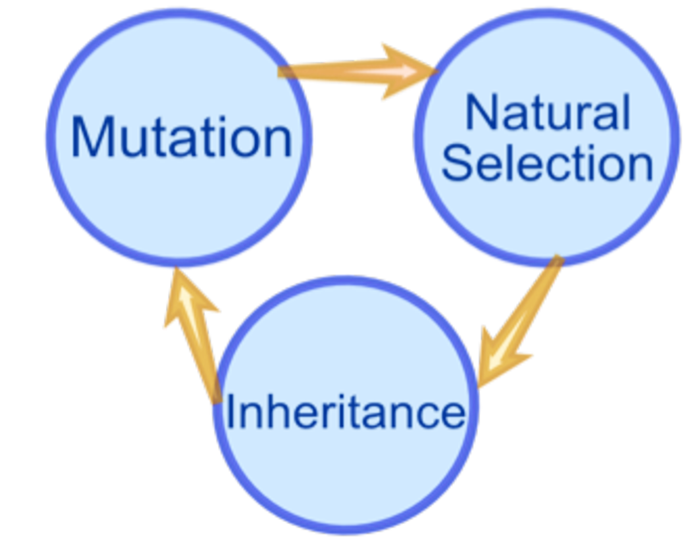
\includegraphics[width=0.43\textwidth,trim={20 19 0 23},clip]{EvolutionCycle}
       \vspace{-20pt}
    \caption{Cycle of evolution towards improved solutions.} 
\label{fg:EvolutionCycle}
  \end{center}
  \vspace{-25pt}
\end{wrapfigure} 
Increasing the speed of progress is a worthwhile goal and so it is instructive to look at how this has been achieved in the broader 
technology sector.  The innovative culture developed within this sector in the last 10 years has propelled it to more rapid innovative progress 
than at any prior time in human history.  One of the critical features of this improvement has been the 
realization that innovation is an evolutionary 
process involving three core functions organized in a feedback loop, as illustrated in Figure \ref{fg:EvolutionCycle}: mutation, 
natural selection, and inheritance. 
In other words, an existing process must be changeable, have a direct path to merit-based survival or death, and retain memory of past 
attempts to avoid repeating mistakes.  The speed of progress is therefore affected by three factors:

\begin{itemize}
\item the intelligence with which any particular function can achieve its goal (i.e. how well mutation chooses the next iteration, possibly 
	using statistical tools such as the open source Metric Optimization Engine \cite{MOE:16}),
\item the speed of transition between functions (e.g. the length of time between natural selection and the next mutation)
\item and the parallelization of cycles (i.e. can multiple mutations be attempted simultaneously or must they operate serially)
\end{itemize}

To speed up innovation, one or more of these factors must be made faster.  This approach reduces to three fundamental properties 
for innovative progress:

\begin{itemize}
\item it must be both cheap and fast to try and fail (more mutations),
\item it must be possible for bad ideas to be properly identified and abandoned quickly (efficient natural selection),
\item and past successes should be easy to incorporate in future innovations (good inheritance).
\end{itemize}

By adapting the latest in computational architectures which have evolved over the last few years (and their associated communication channels), we propose a framework that should improve all three properties to speed agricultural innovation.

\subsubsection{Advances in Computing: Microservices}   

A "perfect storm" of advances in computing architectures in recent years offers a unique opportunity to 
address these fundamental issues in the 
context of agricultural innovation.  As the modern software industry has struggled to achieve scalability in exponentially larger volumes of 
data, traffic, and complexity, some interesting architectural best practices capable of addressing the three properties above have been 
both tried and proven effective in the demands of commercial use.  Primarily, a global community has grown around the idea of 
microservice-based system design. 

Microservices and log-centric architectures \cite{Thones:15,Fernandez-Villamor:10} are at the center of the computational and 
communications strategies of many of today's industry leaders in Internet of Things (IoT), social media, cloud computing, and 
online retailing including LinkedIn, Microsoft, and Amazon. This type of architecture has distinct advantages in performance at large 
scale while preserving simplicity of software development, revision, and large-scale system management. In this proposal, we 
plan to leverage its advantages for agricultural data systems and algorithm dissemination strategies.
	
For purposes of this discussion we define microservices to be small applications with well-defined input and output signals that 
have a single responsibility within a system \cite{Sneps-Sneppe:14}. A complete processing platform is composed of many microservices 
each independently processing the data streams relevant to its task, creating new data streams, and handling specific information requests. 
Microservice coordination and communications between microservices are handled by distributed consensus servers like Zookeeper or 
Etc and message broker technologies such as Kafka \cite{Kafka:16}, RabbitMQ, or ZeroMQ. Some of the advantages of 
microservices relative to traditional monolithic software are:

\begin{itemize}
\item It is simple to update microservices or create new ones by starting them and attaching to the live message broker channel.
\item Systems based on microservices can easily reallocate resources in response to changing loads by simply adjusting the 
	number of running processes of a particular type.
\item Software design is simpler in the microservices architecture because it lends itself to an extremely modular code base. 
	Typical microservices are only a few hundred lines of code \cite{Sneps-Sneppe:14}.
\end{itemize}

The weakness of the microservices architecture which has been overcome in recent years lies in the communications required to 
pass messages and data between them. Typically, complete communications between a group of microservices requires a 
number of service interconnections which is order of the square of the number of services in the group. This centralized 
management of communications between microservices does not scale well and would be untenable in a large system constantly 
adding and removing services in response to computational demand. 

Until relatively recently message passing schemes such as RabbitMQ, ActiveMQ, and ZeroMQ were used to build well-defined 
(though rigid) service interconnections. They all provide strong delivery guarantees, which are used to simplify system design since 
early or ungraceful failure of a particular microservice does not have to result in lost messages. However, to use them in a distributed 
environment requires complicated consensus algorithms, such as Paxos \cite{Lamport:98} or Raft \cite{Ongaro:14}, and more 
often than not they become a performance bottleneck. 
	
In turn, microservice systems have begun to embrace truly stateless service designs that operate without regard of other 
processes in the system, even including other copies of the same service. In general, services should merely react to new data 
events and information requests in the order they are generated. As a result the message broker could be dramatically simplified to a 
basic log-like structure, often referred to as an event service bus, that merely stores messages in the order they are received. 
Kafka \cite{Kreps:11},
LogBus \cite{Vo:12}, 
Amazon Kinesis \cite{Varia:14}, and Azure Event Hub \cite{Machiraju:15}, are all 
examples of highly distributed and highly available implementations of such a log broker.  For example, a small and inexpensive 
three node Kafka cluster is capable of sending and receiving over 2.5 million messages per second and over 249.5 MB of data per 
second \cite{Kreps:14}. LinkedIn's production scale Kafka cluster is capable of sending and receiving over 800 billion messages per day 
which amounts to over 175 terabytes using over 1100 brokers in 60 clusters
\cite{Palino:15}.  This translates to over 63 petabytes per year, 
precisely the data scales of interest in this proposal.

There are significant challenges to designing a modular system comprised of mostly stateless microservices connected to a 
high-throughput event bus, including race conditions (near simultaneous events such that the first one completed cannot be 
communicated quickly enough to the second), unpredictability of message interactions, and many more.  Also, many real-world 
event log-based systems periodically store "snapshots" of state to avoid needing to store an infinite history of messages.  We intend to 
research methods to leverage the strengths of the Open Ag Data Alliance (OADA) project as a means to standardize this state mechanism 
within the microservice architecture, allowing each microservice to choose its own ideal method of interacting with data: either by querying 
current state or as a log of changes that results in the current state.  This proposal is targeted at researching effective best practices 
and new paradigms for agriculture-specific problems, and leveraging the features of microservice system design to enable truly shareable 
algorithms in agriculture.

\subsubsection{Advances in Computing: Containers}   

To complement the appearance of microservice architectures, another recent computing paradigm is transforming the way we think 
about running and deploying software: containers.  Container-based infrastructures are a means of representing an entire running 
machine (operating system, libraries, and software) in such an efficient way that this representation of a machine can run at native speeds 
using few extra resources.  This "container" representation of a machine ensures that the piece of software will run the same, no matter 
where or when it is deployed, because it already contains all the details about software library versions, operating system quirks, etc.   
Note that these containers are a contrast to traditional virtual machines in that they carry little of the storage and computational overhead.  
For example, a recently popular Node.js-based base container \cite{Reeder:16} has a total size of only 25MB, yet represents a complete 
operating system capable of running Javascript processes in Node.

One fundamental problem solved by containers is mitigating the effects of operating system and software library versions changing over time.   
Even though a particular operating system or software library has fallen into disuse, a container originally built with it can be run 
just as it was when the original author created it, with negligible performance penalties due to this virtualization.  

\subsubsection{The Open Source Paradigm}   

Open source software has radically transformed our world in a very short time.  Almost all software and electronic devices in 
existence today owe at least some part of their function to open source code or hardware.  Examples include the Linux kernel, 
Apple?s OS/X and iOS operating systems, Microsoft's .NET framework, Google's Android operating system, the Apache web server, 
and the programming language node.js.  In fact, as of July 2016, there are over 250,000 open source libraries being downloaded over 
1 billion times per week on the popular Javascript code sharing site, Node Package Manager \cite{NPM:16}.

Open source is the means by which the software industry has moved beyond the limits of what fully proprietary, integrated systems 
can achieve.  Unfortunately, the current scenario in agriculture, both in industry and academia, is ruled largely by closed or incompatible 
systems and datasets. The key to enabling agriculture to expand the data frontier is the creation of open source communities of 
developers and researchers that can organically work together, regardless of physical location, on projects and code that have 
direct interest to the participants. 

A paradigm has emerged with best practices for open source projects in the last several years.  Code is generally hosted on the free 
code collaboration site Github, which provides each repository with free web hosting, a project wiki, a powerful issue tracker, and other 
community management features.  We will follow this open source paradigm with the work in this proposal: code and data will be publicly 
available both during development and after, a mailing list and public Slack channel will be utilized for team communication, and proper 
documentation will be included with all algorithms as instructions for others to use the code.  Links to these resources will be printed in 
all resulting publications.  Tutorials, instructional videos, and a "Getting Started" guide will all be available via a project website.

\subsection{On-going and Recent Related Activities}

\subsubsection{Computing: Open Ag Data Alliance}   

The Open Ag Data Alliance was introduced in March 2014 by the Purdue Open Ag Technology and Systems (OATS) 
Group to create an open source common Application Programming Interface (API) for securely and automatically moving 
data between cloud systems and agricultural applications. At this time OADA has grown to 25 commercial partners on 3 
continents. Its technical accomplishments include:

\begin{itemize}
\item The definition of a flexible REpresentational State Transfer (REST) API \cite{Ault:15a}.  REST APIs have 
	become the global standard by which data is communicated among most digital systems after its original introduction
	\cite{Fielding:00} and subsequent distribution as the core architectural style of the internet.
\item A complete open source distributed identity federation \cite{Ault:15b}.
\item The demonstration of data exchange over the API between 5 different partners spanning two continents and three countries. 
\item The creation of an automated conformance test suite in concert with industrial partners seeking OADA conformance certifications.
\end{itemize}

The project hosts all its code publicly in Github (https://github.com/oada), and maintains an active website at http://openag.io.  
The group expects several partners to have the first commercially-available OADA-conformant services in place by the end of 2016.
The OADA vision is one where, once proper permission is granted, the movement, aggregation, anonymization, and synchronization 
of data is automatic.  For example, a farmer can download a new app for weed management, give the app permission to read his/her 
herbicide application records on any OADA-conformant cloud, and the app can immediately give recommendations based on 
past activity. The possibilities are limitless for tools that can exist once there is a standard way to access, synchronize, permission, 
and semantically understand agricultural data in a distributed context.
 
\subsubsection{Autogenic Metadata Sensing and App Development}   

Over the last several years the Purdue OATS research group has been investigating open source software and 
hardware specifically related to autogenic data -- data generated automatically or autonomously with semantic meaning 
due to context. This was funded in part by a USDA-NIFA grant. A suite of apps were developed and posted on GooglePlay. 
They facilitate management and logistics by tracking, at the field level, assignments, activities, and progress and have 
been incorporated into instructional programs and used on research farms \cite{Welte:14a,Welte:14b}. Though the apps were 
designed primarily for logistics they also facilitate communication and data flow ensuring the capture of context in 
agricultural research and production settings.

 The most recent development with the autogenic project has been a "manure app" \cite{Koester:15}.  Manure app is indeed 
autogenic. After set-up and configuration it will autonomously generate complete records of manure application, aggregated 
at the load level.  An inexpensive Bluetooth-enabled ID tag with accelerometers (TI CC265) enables automatic inference 
of the spreader identity and on/off status.  This approach to metadata sensing would be very easily adapted to other 
agricultural operations such as spraying, planting, tillage, scouting, and even harvest of "batch collected" or baled 
commodities such as tomatoes, apples, or forages. 
	 
\subsubsection{ISOBlue and CANDroid: Machine Data to the Cloud for Ag Internet-of-Things}   

The Purdue OATS group has designed and released the ISOBlue hardware/software package which accesses the 
Controller Area Network (CAN) bus of an agriculture or forestry machine through a standard diagnostic port. CAN 
data is streamed to a mobile device through a Bluetooth connection and then can be stored in the cloud \cite{Layton:14}. 
The latest version, dubbed "CANDroid", runs on an Android tablet with only a CAN-to-USB converter (Figure \ref{fg:CANDroid}).
Relevant to this proposal?s focus on microservice architectures, we recently used a Kafka event bus to integrate 
CANDroid live message streaming into an OADA API for delivery to mobile apps, as shown in Figure \ref{fg:CANDroid-Microservice}.  

This is an 
excellent example of the type of architecture described in this proposal.  The CANDroid device places each message on the 
Kafka event bus in the cloud in real-time as it is generated from the machine.  This is an example of a "Collector" 
microservice described in Section 3.  A "GPS Parsing" microservice ignores all messages except those containing 
GPS data, and it transforms the original machine messages into Latitude, Longitude, Altitude, and time, putting a new 
message back on the bus.  A separate "Fuel Rate Parser" microservices does the same.  Each of these are examples 
of "Transformer" microservices described in Section 3.  The "Fuel Rate Map Creator" microservice (an example of 
a "Miner" microservice described in Section 3) watches the bus for GPS and Fuel rate messages with timestamps, 
and aligns them to create fuel rate map messages composed of a fuel rate at a particular GPS location.  Finally, this 
information is organized into geospatial tiles and put into an OADA server to be available in real-time to any connected 
mobile devices for analysis and viewing on a map (an example of a "Visualizer" microservice described in section 3).  
Note that this architecture is scalable and fault tolerant: more data can be handled simply by spinning up more of 
any particular microservice, and unexpected service failures do not result in cascading overall system failure.  

\begin{figure} 
\centerline{
\begin{tabular}{cc}
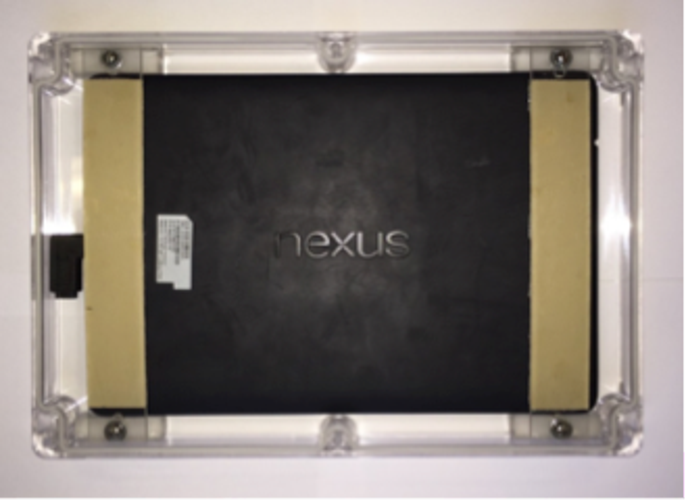
\includegraphics[width = 0.4\textwidth]{Nexas9} & 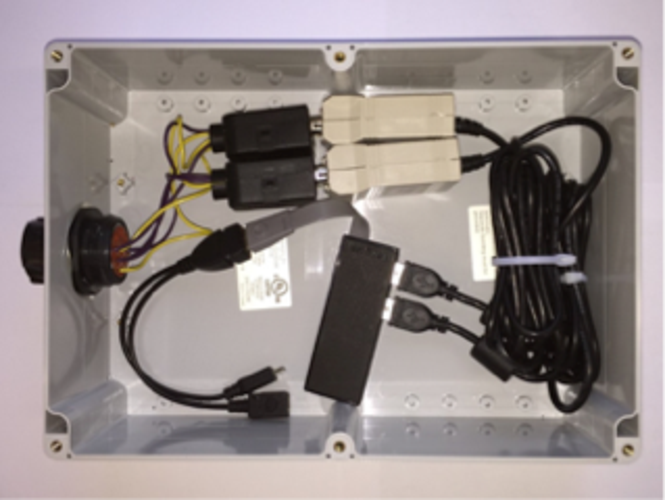
\includegraphics[width = 0.4\textwidth]{Cables} \\
(a) & (b)
\end{tabular}
}
\caption{CANDroid device enclosure's top panel with the (a) Nexus 9 fastened onto the panel and (b) internal USB
	converters, hub, and power connections.} 
\label{fg:CANDroid}
\end{figure} 

\begin{figure} 
\centerline{
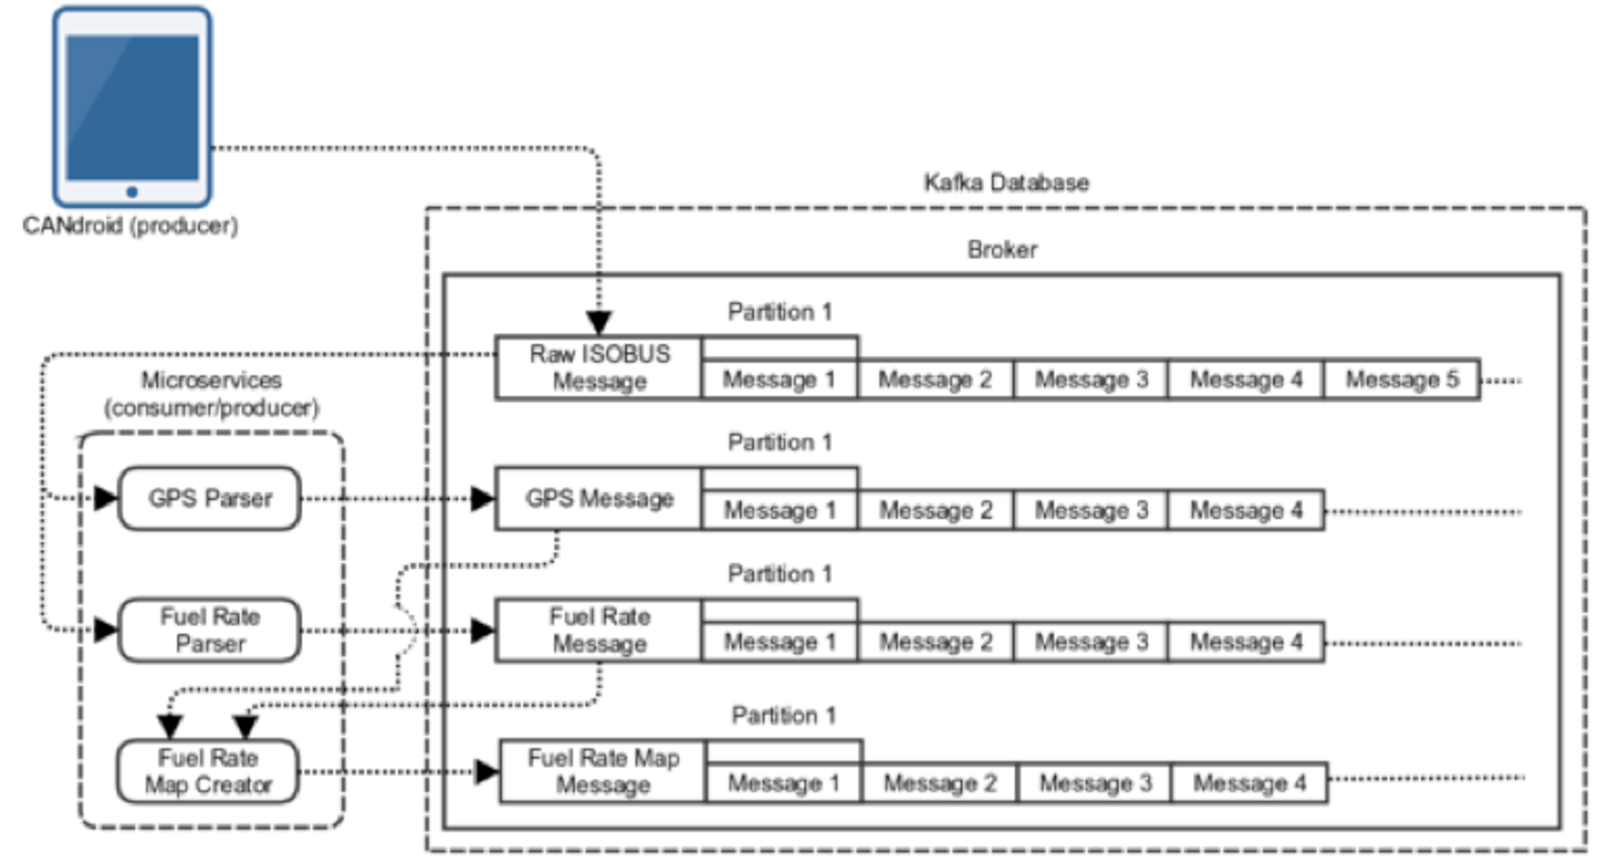
\includegraphics[width = 0.8\textwidth]{CANDroid-Microservice}
}
\caption{CANDroid microservice-based communications architecture.} 
\label{fg:CANDroid-Microservice}
\end{figure} 

\subsubsection{Parallel Supercomputing Cluster}   

Members of the proposal team have built a testbed in prior work which is able to exploit the multiple-scale parallelism 
provided by modern multiple-core general purpose processors, graphics processing units, and FPGAs to leverage modern 
cloud computing development tools. The testbed represents a cloud supercomputing cluster connected to the analog 
continuous-time world by high-performance analog-to-digital and digital-to-analog conversion (see Figure \ref{fg:IoT-testbed}.) The general 
purpose servers provide in total 800 cores via hyperthreading. Several TBs of fast (PCIe connected) flash memory is 
available to the cluster.  
For purposes of this proposal, this infrastructure will be used to effectively test architectures at scale to determine 
data throughput, latency and processing requirements and to evaluate fault tolerance.

\begin{figure} 
\centerline{
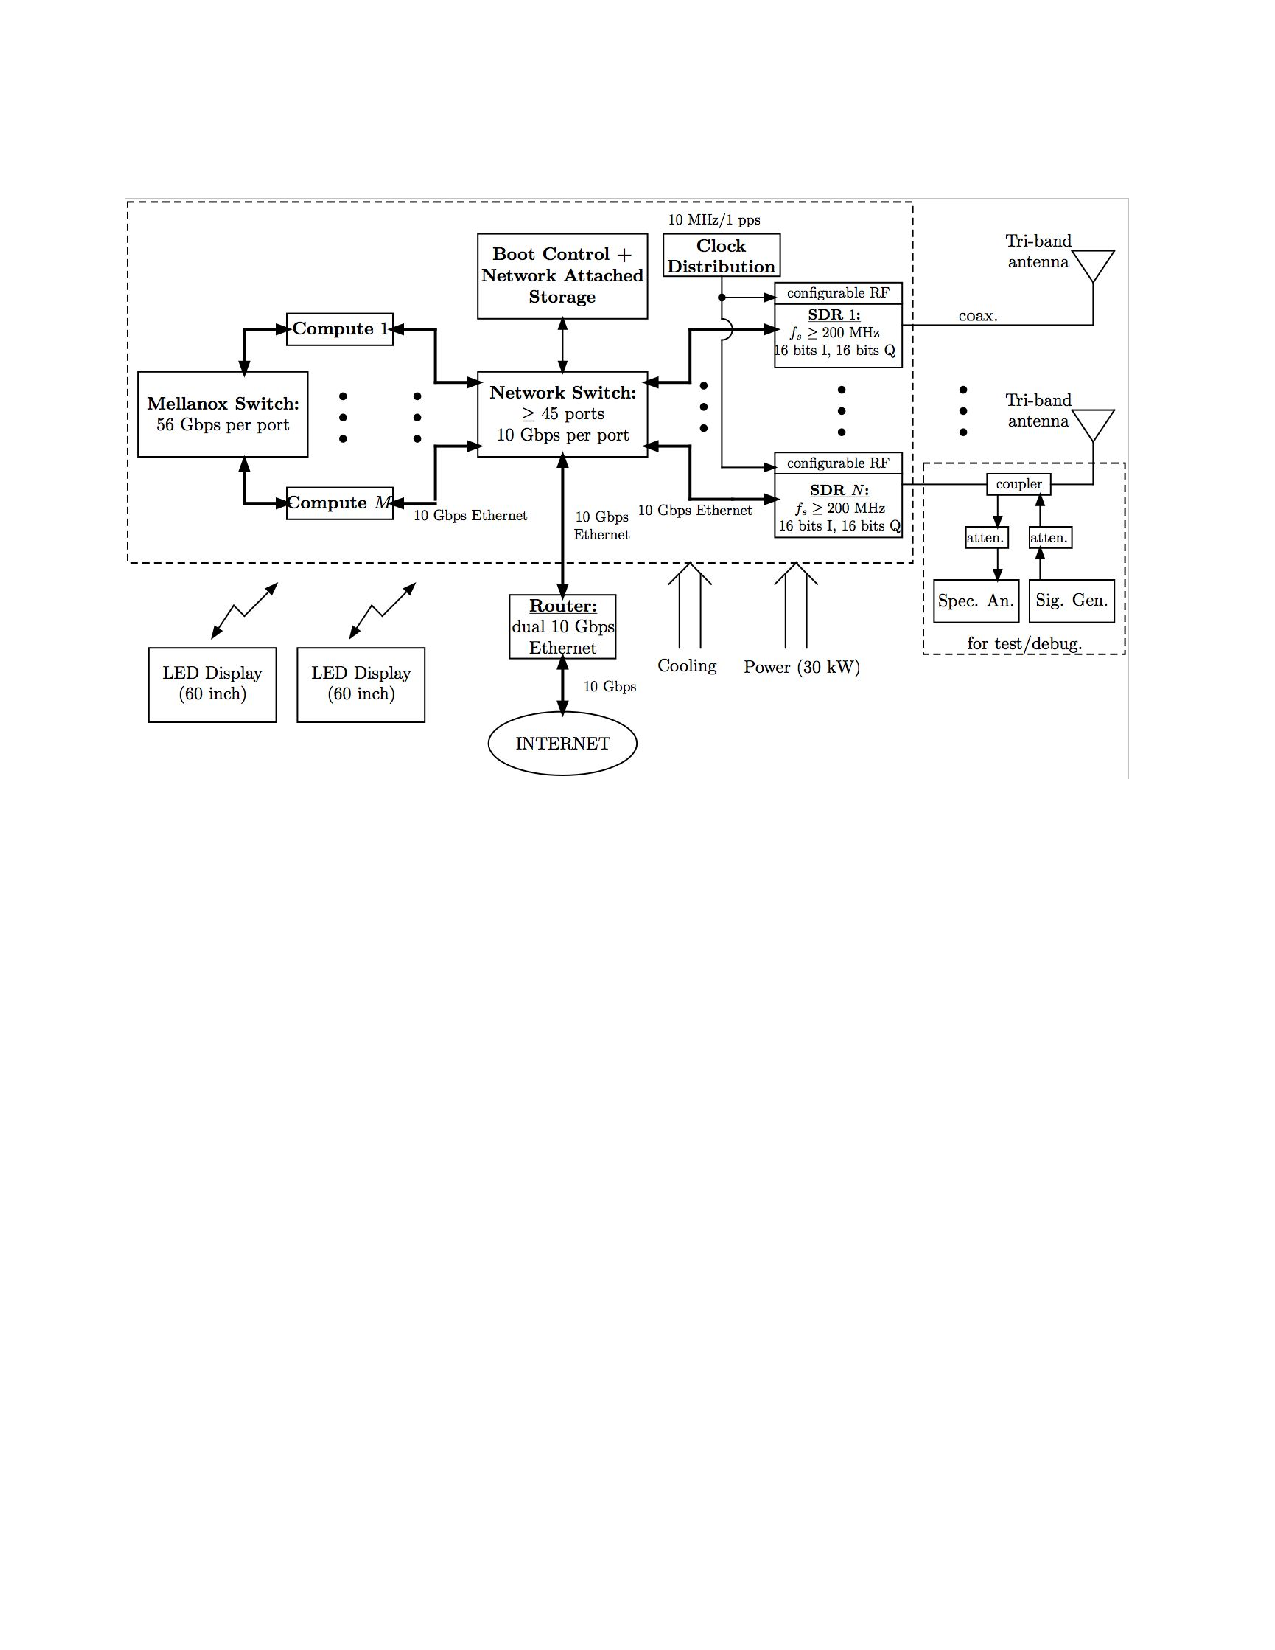
\includegraphics[width = 0.8\textwidth]{CloudRadioFigure}
}
\caption{Purdue testbed for multiscale parallel computing.} 
\label{fg:IoT-testbed}
\end{figure} 

\subsubsection{Computing: Data Visualization}   

The TrialsTracker app \cite{TrialsTracker:16} is an open-source mobile application for farmers, agronomists, and 
other stakeholders to record notes about their on-farm trials which may then be evaluated at the time of harvest. 
Through a simple note-taking interface, users describe the trial before drawing a polygon of the trial area on the map; they 
may then tag these trials with their own custom descriptors for categorization of their yield data comparisons.  The app can compare yield 
(or any other data layer) statistics and the differences between two geospatial regions of interest (part of a field compared to the 
whole field, field 1 compared to field 2, etc.). Rather than the conventional grower-farm-field structure of agricultural field data, 
data is stored in spatially similar geohash buckets; these geohash buckets streamline the visualization and statistical 
comparisons as tiles with aggregation appropriate to the zoom level are loaded and displayed according to the 
applicable geohash level (Figure \ref{fg:TrialsTracker}). 
They also facilitate cross-platform usage of geo-referenced data. With geohashes of differing length driving the tile display, 
data can be quickly displayed as the user might zoom from a few square meters to several square miles -- just like 
satellite imagery in mapping applications. The data is synced with an OADA server, allowing for real-time data visualization 
and evaluation of data as it enters the event bus (such as at the time of harvest).

\begin{figure} 
\centerline{
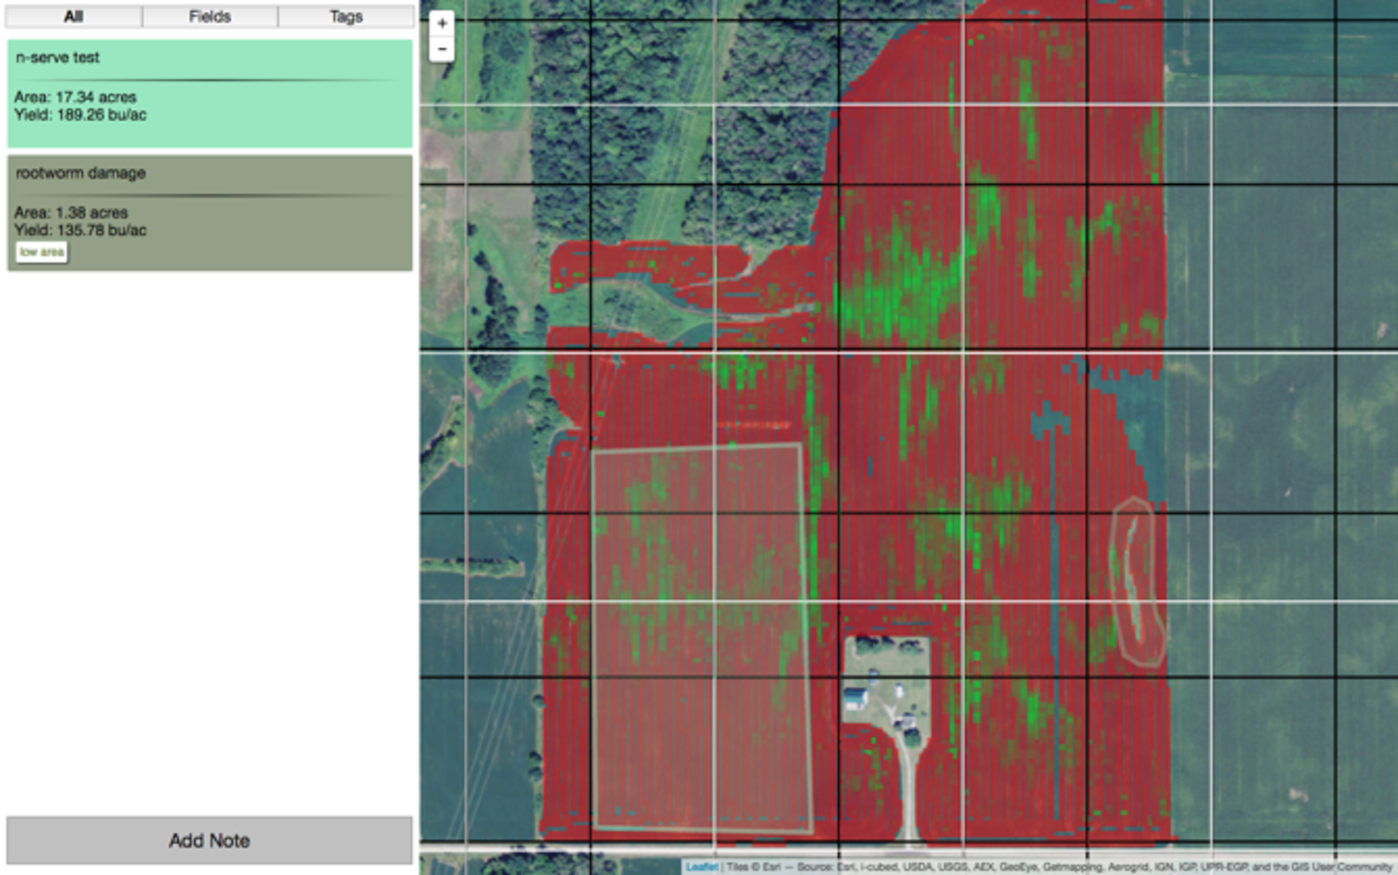
\includegraphics[width = 0.8\textwidth]{TrialsTracker}
}
\caption{TrialsTracker app (white grids are tiles, black grids are geohash buckets of small chunks of data.} 
\label{fg:TrialsTracker}
\end{figure} 
	
\section{Rationale and Significance}

\subsection{Rationale}

The focus of this effort is to leverage current computational approaches to develop and demonstrate an 
engineered system which can assist in meeting both agronomic and management needs in agricultural 
research and production agriculture.  To seamlessly collect, transform, mine, and visualize agricultural data 
(both private and public) at large scale will require a major shift in infrastructure. Privacy, security, data quality, 
and context issues are also important and addressable in the proposed framework, although they are 
not the focus of this proposal.

\subsection{Relationship to Program Area Priorities}

This proposal to demonstrate a scalable algorithm sharing framework is a direct application of scientific 
and mathematical principles to engineer technologies, tool, processes, and systems for it addresses several 
program area priorities, namely:

\begin{itemize}
\item Automation and information systems (with special application to plant production and protection most immediately)
\item Develop tools and technologies for monitoring, measurement, and detection in agricultural systems 
	(indirectly by making data from these systems more accessible and interpretable)
\item Create a roadmap for the next generation of agricultural technologies, particularly in the areas of 
	cyber-physical systems and information management
\end{itemize}

\subsection{Larger Impacts}

Phenomics has gained tremendous traction over the past couple years as a tool for improving plant 
breeding and genetics. Some have observed, however, that knowledge of physical traits has long been 
and continues to be a management tool, as well.  This project is not solely related to phenotyping, but the 
framework and infrastructure model will be very applicable as data streams in agriculture increase by 
orders of magnitude due to imaging and additional sensors.

Greater utility of both public and private data requires easier access and more flexible architectures 
for collecting, transforming, mining, and visualizing this data. Many of the processes needed can be 
learned by artificial intelligence systems (neural nets, etc.), but familiarity and access to these tools 
requires a culture shift toward open-source projects such as this one.

Another larger impact of this proposed work is the improved speed of innovation and refinement 
with regard to crop production (and other) systems.  While one benefit of a microservices framework is 
improved scalability, it also streamlines innovation and distributed development by isolating large and 
complex analyses into smaller, more comprehensible and shareable elements. This allows experts to 
contribute to algorithms, models, and devices with less requisite knowledge than is needed to 
model ?the whole system?.

\section{Approach}

\subsection{Activities and Sequencing}

\subsubsection{Objective 1: Research microservice-based computing architectures and design a solution for scalable, 
	sharable, real-time agricultural data systems}   
	
The first step will be to formalize the basic architectural components that each microservice can assume 
are part of the framework in which it is running.  Along the lines of typical microservice best practice, 
each microservice should be capable of learning about and adapting to its environment as a means of 
improving manageability and reliability.  Therefore, a core part of the framework will be the means by which 
each microservice can achieve this, and corresponding open source code implementing that framework.  

The research team has solved similar problems to this in the past as part of their work designing the 
Open Ag Data Alliance REST API, and many of the same solutions can apply in this context as well.  
For instance, a client application to an OADA-based cloud service can learn everything it needs about 
the cloud service by retrieving a cacheable domain configuration document at a standard location, discover 
the location of resources using the OADA-defined "/bookmarks" endpoint, and later learn the data formats and 
ontologies used by the cloud via content types that are reported with each resource.  

Some of the interesting architectural work here will be around classifying the types of problems, failure 
modes for those problems that are exploitable for performance gains, and stream-based processing 
methods for agriculture-specific data systems.  Some algorithms which appear straightforward as 
monolithic applications can become complex when transformed into stateless services that operate on 
streams of data and make use of the best features of functional programming for parallelizability, 
reliability, and simplicity.

\subsubsection{Validate the research of Objective 1 by building an end-to-end solution focused on monitoring stand 
	establishment and early development in corn... }  

This phase of the project involves first determining the high-level functions necessary to perform the monitoring 
of corn plant emergence and early life development, with a focus on scalability using simulated data.  This design 
work will focus on laying out the particular microservices we will need within the framework from 3.1.1, 
categorized according to the following four classifications:

\begin{enumerate}
\item {\em Microservice Class 1: Collectors.} Collectors are tasked with retrieving external data and placing it into 
	storage locally.  Examples of this class include retrieval of soil information, LiDAR elevation data, 
	NOAA micro rainfall data, and collection of plant health and biomass data from physical sensors.
\item {\em Microservice Class 2: Transformers.} Given local data on the event bus or stored in an 
	OADA service, convert that data into a different form or index it differently.  Examples of this class 
	include transforming NOAA rainfall shapefiles into geospatially-indexed rainfall data, transforming 
	existing LiDAR point cloud data into Digital Elevation Models, reformatting a proprietary binary 
	data files into usable information, etc.
\item {\em Microservice Class 3: Miners.} Using statistics, models or machine learning, produce insights or 
	aggregates generated from existing data.  While it may be difficult to classify a particular algorithm as a 
	Transformer or a Miner given that they both take data as input and produce an output based on that data, 
	Miners differ from Transformers in increased complexity and in the ability to combine multiple sources of data.  
	Examples of Miner microservices include image processing, object recognition, corn growth models, soil 
	erosion models, etc.
\item {\em Microservice Class 4: Visualizers.} Visualizers may run either as containers which pre-process data to 
	make it suitable for visualization, or as the Javascript code designed to run in browsers or mobile apps and 
	display data to an end user as charts, maps, or animations.  Javascript is the most ubiquitous language available, 
	making it an ideal choice for distributable visualization libraries.  The main goal of this class of visualizers is to 
	dramatically simplify the work needed by a researcher or developer to look at data generated by the other 
	three classes of microservices.  Examples of visualizers include pre-processing raw geospatial data into 
	map tiles, libraries for displaying large amounts of geospatial data on mobile devices, charting tools to 
	display results of basic calculations, and many others.
\end{enumerate}

To adhere to the microservice design philosophy of modularity and fault tolerance, the design of each microservice 
will require it to operate to the best of its ability in the presence of either partial information or varying granularity 
of information.  For example, a microservice which needs rainfall data as input should be able to give a best-effort 
output if the input data is a weekly state-wide estimate or if it is a highly-dense on-site network of cloud-connected rain 
gauges.  

The agronomic research topic in this proposal highlights the power of this approach: there are many ways to collect 
indicators of the various data of interest: canopy height, relative plant height, spacing between plants, physiological 
development rate, etc.  Manual measurement and sampling, drone imagery as available, manned aerial imagery, 
instrumentation of farm equipment, a hobby-grade radio controlled vehicle with an open source autopilot system, and 
others are all valid, reasonable means of collecting data.  Any particular method that the project team proposes for 
collecting such information will likely have varying levels of success: some will work well, others will perhaps still 
require manual sampling and input.  The system should be robust enough to produce a result and a confidence 
metric in such a wide variety of eventual situations, enabling the parallel improvement of any particular type of 
data collection, processing, or visualization in its own time.  This design principle maximizes the chances that a 
given microservice will be useful in multiple contexts.  

\subsubsection{Objective 3: Disseminate the algorithms and microservices ...}   

One of the most critical features of a successful open source project is good documentation that can get newly 
interested parties up to speed very quickly.  Such documentation includes tutorials, getting started guides, blog posts, 
and videos.  The project team intends to explicitly focus on this goal in the second half of the project timeline to 
minimize the changes necessary to keep documentation up-to-date with rapidly changing code in the early phases 
of the project, while incorporating other interested developers as early as possible.  It is all too easy in normal 
projects to let the documentation slip in favor of more features, and we intend that this project not fall into that 
trap by making this an explicit objective.

\subsection{Methods}

\subsubsection{Objective 1: Research microservice-based computing architectures?}

\noindent
{\em Activity 1.1. Architectural research}

The team's prior work with the OADA API will be extended to an event bus paradigm creating a similar well-known 
topic where service discovery can take place.  Message types and formats can be communicated via the use of 
Apache Avro \cite{Avro:16} as the basic encoding scheme for event bus messages, combined with similar 
content type structures that already exist within OADA.

In addition to an event bus, each microservice will have access to a local OADA service to retrieve and store 
information locally that can be shared across microservices.  This data store will be assumed by microservices to 
be eventually consistent in order to remain scalable, and therefore Convergent Replicated Data Types \cite{Shapiro:11} 
will be highly preferred in data models.  A microservice that is only interested in events which alter or create some data 
can use only the event bus, but a microservice that is more interested in processing or querying existing data can rely on the 
OADA server to retrieve or store the state of some data, either via the REST API directly or by publishing a request on the 
event bus.  A tight coupling between the OADA server and the event bus will enable seamless transition from 
one to the other by other microservices.

Many other specific architectural details will become necessary as implementation of the framework progresses.  
These details will be incorporated into the published documentation and publications produced about the architecture.  
Mechanisms for coordination, best practices for stateless service design, and templates to ease the creation of new 
types of common microservices will all be important components of this activity.

\noindent
{\em Activity 1.2. Build a container-based implementation using Docker}

Each microservice will be designed to run in a Docker container that can communicate with the OADA service 
and the event bus.  Docker's Compose (Compose, 2016) and Swarm (Swarm, 2016) utilities will be used to build the 
service interconnections between containers, making any instance of the overall system runnable both locally on a 
developer's computer and in a cloud provider such as Amazon Web Services (AWS) or Microsoft Azure.  The end 
result is a system of many services that can be very simply installed and started with only two commands: a "git clone" 
and a "docker-compose start".

\noindent
{\em Activity 1.3. Test scalability and fault tolerance}

The scalability of this system will be evaluated by instrumenting the various components of the system for profiling, 
and simulating real-time actors producing fake data at realistic rates for thousands of farms.  The project team will 
make use of existing supercomputing infrastructure described in Section 1.3.4 to evaluate the design decisions of this 
phase of the project in terms of scability, latency, data integrity, and fault tolerance.  It will also utilize existing open source 
microservice testing utilities such as ChaosMonkey (ChaosMonkey, 2016), a microservice designed to randomly stop 
other microservices in a system in order to evaluate robustness.

\subsubsection{Objective 2: Validate the research of Objective 1 by building an end-to-end solution focused on 
	monitoring stand establishment and early development in corn...}

\noindent
{\em Activity 2.1. Construct data collection platform}

Outfit an inexpensive, ultra-low ground pressure ground robot with Crop Circle (Holland Scientific, 2011) 
optical sensors, still and video cameras to generate a rich data stream to test the infrastructure. This imagery 
and data will be geo-referenced with RTK accuracy; occasional ground-truthing locators will be placed in the field.

\noindent
{\em Activity 2.2.  Architect and build microservice types and their interactions}

The project team currently intends to build many if not all of the following microservices for this proposal:

\begin{itemize}
\item Collectors: 
	\begin{itemize}
	\item Retrieve SSURGO soil data and load into local OADA server for geospatial regions of choice
	\item Retrieve LiDAR elevation data from several of the available public sources
	\item Collect data from the roving Crop Circle equipped robot and store in OADA server
	\end{itemize}
\item Transformers: 
	\begin{itemize}
	\item Convert SSURGO soil output formats into the proper subset of factors likely to affect 
		germination, emergence and stand establishment
	\item Convert optical sensor legacy format data into geospatially-indexed maps
	\item Convert optical sensor output to plant population, plant spacing, plant height and NDVI geospatially-indexed maps
	\end{itemize}
\item Miners:
	\begin{itemize}
	\item Process imagery into stand count, physiological stage, or canopy height estimates using a 
		state-of-the-art open source neural network image processing framework such as Caffe (Caffe, 2016)
	\item Process image and sensor geo-referenced data to identify key sampling points in a field
	\item Process image and sensor data with different wavelength filters to determine which best detect early season NDVI
	\end{itemize}
\item Visualizers:
	\begin{itemize}
	\item Pre-process raw geospatial data into tiles for efficient map display and statistical calculation 
		on mobile devices using the open source algorithms created by the project team for the in-development 
		TrialsTracker open source application (TrialsTracker, 2016)
	\item Efficient synchronization and display of real-time geospatial data based on the popular 
		Leaflet.js mapping framework (Leaflet, 2016) (also created by the project team for TrialsTracker application)
	\item Charting tools to display results of basic calculations (plant height vs. soil moisture at planting, etc.) 
		using D3.js (D3, 2016) or similar charting libraries
	\item Visually show and communicate pre-computed sampling locations on mobile devices while a 
		researcher, agronomist, or or robot ?walks? a field
	\end{itemize}
\end{itemize}

\noindent
{\em Activity 2.3. Quantify success of corn plant emergence and stand establishment}

?.

\subsubsection{Disseminate the algorithms and microservices ...}

\noindent
{\em Activity 3.1.Code and Project management}

The codebase for the project will reside in the Open Ag Toolkit github project (OpenATK, 2016), maintained by 
the project team as a result of prior USDA funding (GRANT 10867241).  Each microservice will have its own 
repository in that project, complete with issue tracking, documentation, and communication channels for 
developers.  A roadmap for development will be maintained in a new website specific to this project.  A mailing 
list and public Slack team will be created for all developer communication.  In this way, both design decisions 
and the code implementing those decisions will be publicly available from the first day and indefinitely after the 
project completes.

\noindent
{\em Activity 3.2 Development of Documentation}

The proposal team will produce simple video introductions, written tutorials, and extensive documentation 
within the codebase in order to maximize the ability of others to learn about the code and contribute to the 
open source effort.  In addition, a website will be maintained for the project in Github Pages.

\noindent
{\em Activity 3.3 Optimizing Installation and Code Distribution}

It is important once the base framework and individual microservices have been developed that the installation 
procedures be optimized for other researchers not necessarily as well versed in computing as the original 
developers.  The Node Package Manager (npm) (NPM, 2016) provides an excellent demonstration of this 
within the Javascript community.  All Javascript-based code will be released as packages via npm.  In addition, 
all Docker images will be released via the free Docker image sharing service Dockerhub.  The single-line 
commands necessary to install and run each item will be documented, and any areas of installation which 
appear too complex will be a focus for improvement.

\subsection{Expected Outcomes and Deliverables}

Aligning with the long-term goal and project objectives, key project outcomes will be a framework for algorithm 
sharing which incorporates a microservices approach. Design with containers in mind will improve long-term 
stability of solutions for agriculture and the microservices model should improve the speed at which innovation 
in agricultural algorithm and data innovation can occur. Specific deliverables will include sample microservices 
and algorithms, paired with data sets which are available open-source; these will be directly related to corn 
production since the focus is on establishment and uniformity during early stage growth. This code, however, 
should be readily adaptable to other uses of similar data whether for field crops, horticultural crops, or 
any large geo-referenced data sets.

\subsection{Evaluation: Analyzing, assessing, and interpreting results...}

\subsubsection{ ? of the microservices}   

Each microservice will be formally evaluated with the following criteria:

\begin{itemize}
\item Robustness to failure of itself and other copies of itself.
\item Robustness to failure of other microservices.
\item Ability to function with varying resolutions of input information.
\item Response latency (i.e. time from input appearance to output messages)
\item Additional storage required
\end{itemize}

\subsubsection{ ...of the agronomic study}   

The accuracy of automated methods for the determination of successful stand establishment, such as image 
analysis tools for quantifying initial plant emergence, stand uniformity, and phenological development rate will 
be evaluated based on manual measurements. Accurate geo-reference of utility vehicle tracks used to impose 
emergence delay (with mild compaction) will be compared to emergence and plant stage (at various dates) to 
validate the identification and location of variation in plant states. The factors affecting measurement accuracy, the 
amount of time needed and quantity of data generated, and feasibility under diverse field environments will be 
identified. Some analysis of the gains in confidence earned with larger data sets will be conducted.
 
\subsubsection{ ...of the overall framework}   

The overall framework has two main goals: to be an effective guide for the ag data system designs of the 
near future, and to be an effective means of algorithm sharing in agriculture.  To that end, the overall system 
will be evaluated according to the following metrics:

\begin{itemize}
\item Scalability: theoretical limits on system capacity in terms of data size, latency requirements, network bandwidth, 
	and cost per level of scale in commodity cloud platforms.
\item Modularity: each major function of the overall system will be evaluated for dependencies on other parts of the system.  
\item Learning Curve: the knowledge acquisition necessary to build a single microservice will be 
	described and targeted in tutorials, both for a typical ag-based graduate student level and a computer 
	science graduate student level.
\end{itemize}



\newpage

\setcounter{page}{1}

\bibliographystyle{IEEEtran}
\bibliography{JVK_refs}



\end{document}



